\documentclass[11pt, titlepage]{article} 

\usepackage{geometry}
\geometry{left=0.8in, right=0.8in, top=0.8in, bottom=0.8in}

\usepackage{color}
\usepackage{graphicx} % slike
\usepackage{caption}
\usepackage{subcaption}
\usepackage{siunitx} % enote
\usepackage{amsmath} % enačbe
\usepackage{amssymb} % simboli
\usepackage[thinc]{esdiff} % za odvode
\usepackage[colorlinks=true]{hyperref} % za linke
\usepackage{float} % za fiksiranje figur
\usepackage{mathtools}
\usepackage{esint} % za fancy integrale
\usepackage[numbib,nottoc]{tocbibind}
\usepackage[slovene]{babel}
\usepackage{diagbox}

\usepackage{tikz}

\newcommand{\dif}[1]{\,{\rm d}#1}

\begin{document}

\begin{titlepage}
    \begin{center}
        \includegraphics[width=0.5\textwidth]{figures/FRI_logo.png}\\
        \vspace{0.5cm}
        \vspace{3cm}
        {\LARGE \bf Obhod Lune} \\
        \vspace{0.3cm}
        \vspace{2.0cm}
        {\large Numerična matematika}\\
        \vspace{0.2cm}
        {|}\\
        \vspace{0.2cm}
        {\large 3. domača naloga}\\
        \vspace{2.0cm}
    \end{center}
    \vfill
    \begin{flushleft}
        {\normalsize {\sf Avtor:} Vito Levstik\\}
    \end{flushleft}
    \vspace{2cm}
    \begin{center}
        {\normalsize \sc Akademsko leto 2024/2025}
    \end{center}
\end{titlepage}

\newpage

\section{Uvod}

Cilj naloge je simulacija potovanja vesoljskega plovila okoli Lune na tiru z vrnitvijo brez potiska.
Rešujemo omejen krožni problem treh teles, kjer je masa plovila zanemarljiva v primerjavi z maso Zemlje in Lune.
Enačbe gibanja rešujemo v vrtečem se koordinatnem sistemu, v katerem Zemlja in Luna mirujeta. Rešiti moramo torej sistem 
\begin{align*}
\ddot{x} &= x + 2\dot{y} - \frac{1 - \mu}{R^3}(x + \mu) - \frac{\mu}{r^3}(x - (1 - \mu)) \\
\ddot{y} &= y - 2\dot{x} - \frac{1 - \mu}{R^3}y - \frac{\mu}{r^3}y \\
\ddot{z} &= - \frac{1 - \mu}{R^3}z - \frac{\mu}{r^3}z
\end{align*}
kjer je $R = \sqrt{(x + \mu)^2 + y^2 + z^2}$ in $r = \sqrt{(x - (1 - \mu))^2 + y^2 + z^2}$ razdalja do Zemlje in Lune.
Parameter $\mu$ je definiran kot $\mu = \frac{m}{M+m}$, kjer je $m$ masa Lune, $M$ pa masa Zemlje, kar nam da približno vrednost $\mu = 0.01215$. V brezdimenzijskih koordinatah je Zemlja v točki
$(-\mu, 0, 0)$, Luna pa v točki $(1 - \mu, 0, 0)$.

\section{Implementacija}
Definiramo vektor stanja $X = (x, y, z, \dot{x}, \dot{y}, \dot{z})$. Njegov odvod je tako $\dot{X} = (\dot{x}, \dot{y}, \dot{z}, \ddot{x}, \ddot{y}, \ddot{z})$, kjer poznamo eksplicitne izraze za $\ddot{x}$, $\ddot{y}$ in $\ddot{z}$.
Nalogo rešimo iterativno s pomočjo Runge-Kutta metode 4. reda, ki vsak naslednji korak izračuna kot
\begin{align*}
k_1 &= h \cdot f(t_n, X_n) \\
k_2 &= h \cdot f(t_n + \frac{h}{2}, X_n + \frac{k_1}{2}) \\
k_3 &= h \cdot f(t_n + \frac{h}{2}, X_n + \frac{k_2}{2}) \\
k_4 &= h \cdot f(t_n + h, X_n + k_3) \\
X_{n+1} &= X_n + \frac{1}{6}(k_1 + 2k_2 + 2k_3 + k_4)
\end{align*}
kjer je $f(t, X)$ funkcija, ki vrača odvod vektorja stanja $X$ ob času $t$ in $h$ velikost koraka. Metodo smo implementirali v funkciji \texttt{rk4\_method}, ki sprejme začetni vektor stanja, časovni korak in število iteracij. Na vsakem koraku funkcija dodatno preveri,
če je plovilo trčilo v Luno ali Zemljo in predčasno konča simulacijo, če je prišlo do trka. Za Zemljo in Luno smo privzeli, da sta popolni krogli z radijema $R_Z = 6400 \text{ km}$ in $R_L = 1700 \text{ km}$.

Najtežji del naloge je izbor začetnih vrednosti, saj želimo najti orbite z vrnitvijo brez potiska, kar se zgodi le v redkih primerih.
Na sliki \ref{fig:theory_orbits} so prikazane orbite, dobljene iz literature, ki jih želimo v tej nalogi reproducirati.
\begin{figure}[h]
    \centering
    \begin{subfigure}[b]{0.45\textwidth}
        \centering
        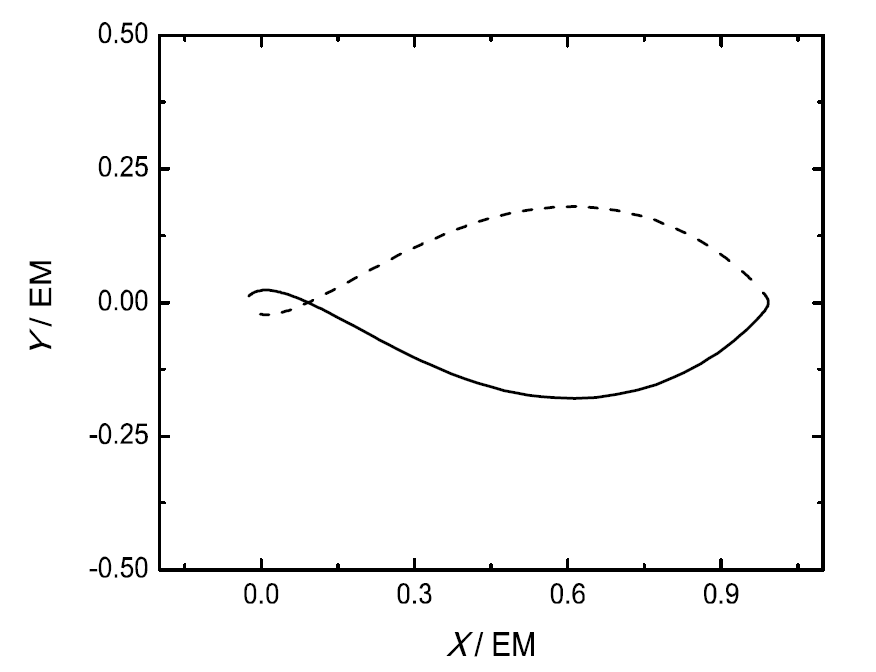
\includegraphics[width=\textwidth]{figures/theory_orbit_1.png}
        \caption{Progradna orbita z začetkom na nasprotni strani Zemlje kot Luna.}
        \label{fig:orbit_1}
    \end{subfigure}
    \hfill
    \begin{subfigure}[b]{0.45\textwidth}
        \centering
        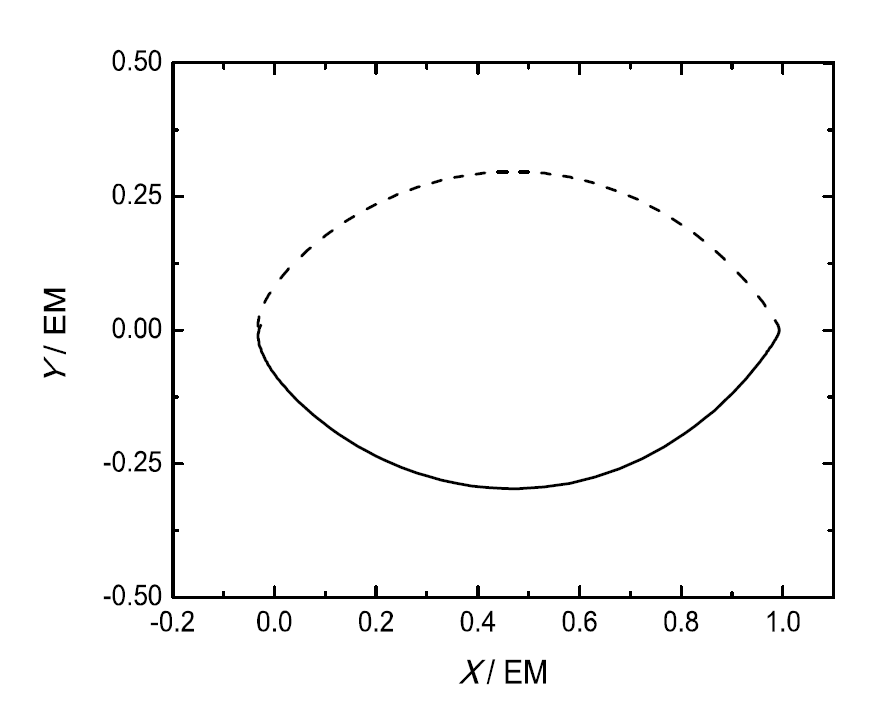
\includegraphics[width=\textwidth]{figures/theory_orbit_2.png}
        \caption{Retrogradna orbita z začetkom na nasprotni strani Zemlje kot Luna.}
        \label{fig:orbit_2}
    \end{subfigure}

    \vspace{0.5cm}

    \begin{subfigure}[b]{0.45\textwidth}
        \centering
        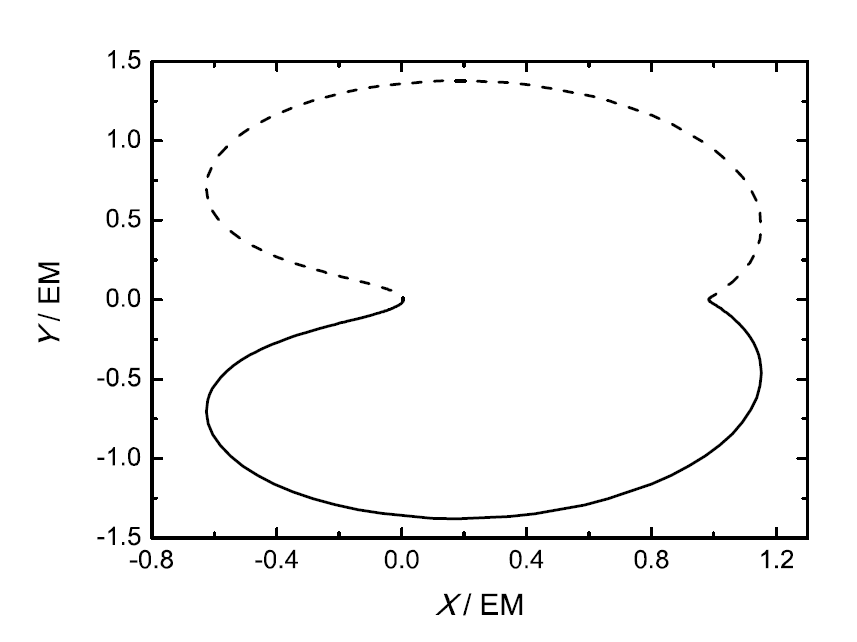
\includegraphics[width=\textwidth]{figures/theory_orbit_3.png}
        \caption{Progradna orbita z začetkom na isti strani Zemlje kot Luna.}
        \label{fig:orbit_3}
    \end{subfigure}
    \hfill
    \begin{subfigure}[b]{0.45\textwidth}
        \centering
        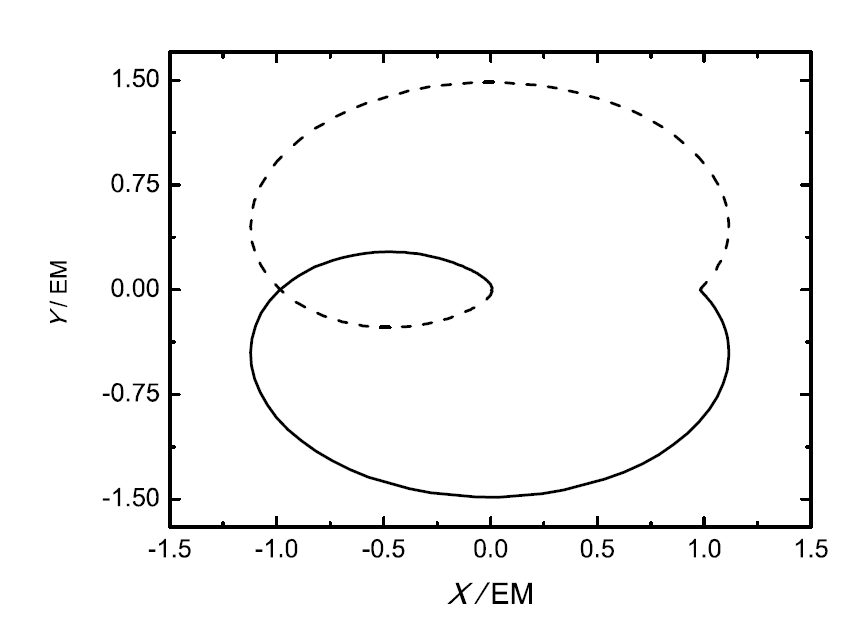
\includegraphics[width=\textwidth]{figures/theory_orbit_4.png}
        \caption{Retrogradna orbita z začetkom na isti strani Zemlje kot Luna.}
        \label{fig:orbit_4}
    \end{subfigure}

    \caption{Orbite, dobljene iz literature.}
    \label{fig:theory_orbits}
\end{figure}

\section{Rezultati}
Tekom simulacij se omejimo na gibanje v $xy$ ravnini. Takšna obravnava je smiselna za majhne odmike $z$.
Za majhne odmike $z$ sta $R$ in $r$ funkciji le $x$ in $y$, torej lahko pišemo
$$
\ddot{z} = - a^2 \cdot z,
$$
kjer definiramo $a^2 = \frac{1 - \mu}{R^3} + \frac{\mu}{r^3}$. Dobimo enačbo harmoničnega nihanja, katere rešitev je
$$
z(t) = A \cos(at) + B \sin(at),
$$
kjer sta $A$ in $B$ konstanti, določeni iz začetnih pogojev. Gibanje v $z$ komponenti bo tako podobno harmoničnemu nihanju, ki se mu sproti spreminja frekvenca nihanja. 

Veliko vesoljskih plovil je izstreljenih iz nižje Zemljine orbite (Low Earth Orbit), zato smo privzeli, da je plovilo izsteljeno iz višine $200 \text{ km}$ nad površjem. Vektor hitrosti plovila je v tem trenutku pravokoten na vektor pozicije, relativno na središče Zemlje. Iskanje ustreznih začetnih pogojev
je tako omejeno na iskanje začetnega kota $\alpha$ (merjen od zveznice med Zemljo in Luno v pozitivni smeri) in velikosti hitrosti plovila $v_0$. S poiskušanjem različnih kombinacij smo našli željene štiri orbite. Pri tem smo želeli doseči, da se plovilo med letom čimbolj približa Luni, za katero smo vzeli, da ima polmer $1700 \text{ km}$. Parametri začetnih pogojev
so prikazani v tabeli \ref{tab:initial_conditions}.
\begin{table}[h]
    \centering
    \begin{tabular}{|c|c|c|c|c|}
        \hline
        \textbf{Št.} & $\alpha$ [°] & $v_0$ & $d_L$ [km] & $t$ [dni] \\
        \hline
        1 & 227.3 & 10.6459 & 1768.5 & 5.687\\
        2 & 210 & -10.6823 & 1867.7 & 5.665\\
        3 & -5 & 10.64555 & 1842.7 & 27.46\\
        4 & 30 & -10.68257 & 1774.8 & 30.84\\
        \hline
    \end{tabular}
    \caption{Začetni pogoji za iskane štiri orbite, minimalna dobljena razdalja do Lune med simulacijo in čas potovanja. Enote za hitrost so brezdimenzijske.}
    \label{tab:initial_conditions}
\end{table}
Enote za hitrost v tabeli \ref{tab:initial_conditions} so brezdimenzijske. Razdalja med Zemljo in Luno je v brezdimenzijskih enotah 1, kar ustreza približno $384400 \text{ km}$. Podobno je kotna hitrost vrtenja sistema enaka 1. 
Ko uporabimo dejstvo, da je perioda vrtenja Lune okoli Zemlje približno $2.36 \cdot 10^6 \text{ s}$, dobimo, da je brezdimenzijska enota hitrosti enaka $1.023 \text{ km/s}$.
Da dobimo hitrosti v realnih enotah, moramo brezdimenzijske hitrosti pomnožiti s to vrednostjo.

Na sliki \ref{fig:orbits} so prikazane orbite, dobljene z uporabo začetnih pogojev iz tabele \ref{tab:initial_conditions} in z uporabo časovnega koraka $h = 10^{-6}$.
\begin{figure}[h]
    \centering
    \begin{subfigure}[b]{0.45\textwidth}
        \centering
        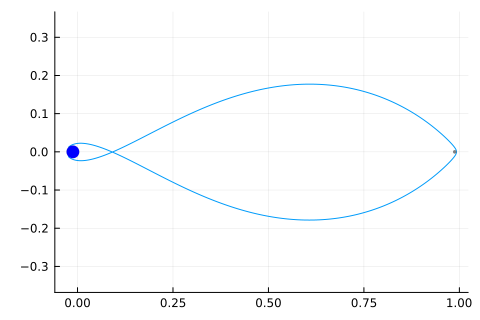
\includegraphics[width=\textwidth]{figures/free_return_orbit_1.png}
        \caption{Progradna orbita z začetkom na nasprotni strani Zemlje kot Luna.}
        \label{fig:orbit_1_sim}
    \end{subfigure}
    \hfill
    \begin{subfigure}[b]{0.45\textwidth}
        \centering
        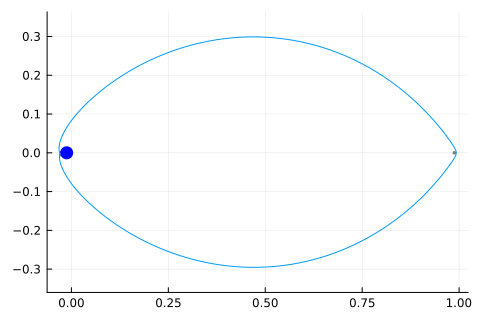
\includegraphics[width=\textwidth]{figures/free_return_orbit_2.png}
        \caption{Retrogradna orbita z začetkom na nasprotni strani Zemlje kot Luna.}
        \label{fig:orbit_2_sim}
    \end{subfigure}

    \vspace{0.5cm}

    \begin{subfigure}[b]{0.45\textwidth}
        \centering
        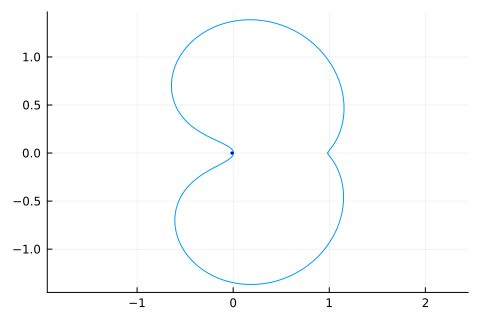
\includegraphics[width=\textwidth]{figures/free_return_orbit_3.png}
        \caption{Progradna orbita z začetkom na isti strani Zemlje kot Luna.}
        \label{fig:orbit_3_sim}
    \end{subfigure}
    \hfill
    \begin{subfigure}[b]{0.45\textwidth}
        \centering
        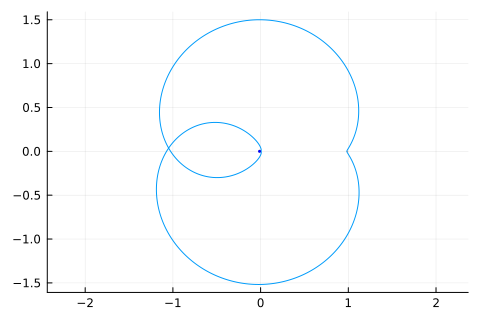
\includegraphics[width=\textwidth]{figures/free_return_orbit_4.png}
        \caption{Retrogradna orbita z začetkom na isti strani Zemlje kot Luna.}
        \label{fig:orbit_4_sim}
    \end{subfigure}

    \caption{Simulirane orbite z uporabo začetnih pogojev iz tabele \ref{tab:initial_conditions}.}
    \label{fig:orbits}
    
\end{figure}
Velikost koraka $h$ določa natančnost simulacije. S preizkušanjem različnih vrednosti ugotovimo, da za prevelike vrednosti (nad $10^{-5}$) pride do kritičnih napak. Plovilo bodisi trči v Luno, ali pa se ne vrne na Zemljo.
Iz tega razloga preverimo kako se končne koordinate plovila spreminjajo za vrednosti koraka $h$ manjše od $10^{-5}$. Rezultati so prikazani na sliki \ref{fig:step_size}.
\begin{figure}[h]
    \centering
        \begin{subfigure}[b]{0.45\textwidth}
        \centering
        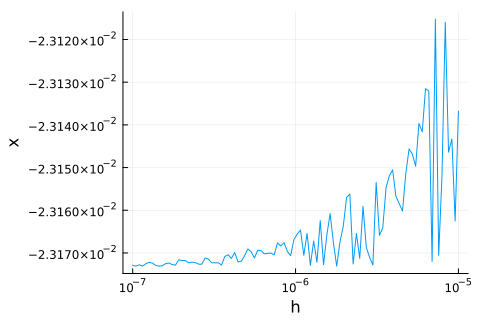
\includegraphics[width=\textwidth]{figures/x_coordinate_vs_dt.png}
        \caption{Končna koordinata $x$ plovila glede na velikost koraka $h$.}
        \label{fig:x_coordinate_vs_dt}
    \end{subfigure}
    \hfill
    \begin{subfigure}[b]{0.45\textwidth}
        \centering
        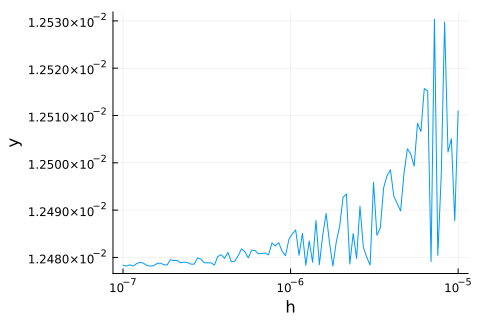
\includegraphics[width=\textwidth]{figures/y_coordinate_vs_dt.png}
        \caption{Končna koordinata $y$ plovila glede na velikost koraka $h$.}
        \label{fig:y_coordinate_vs_dt}
    \end{subfigure}

    \caption{Končne koordinate plovila glede na velikost koraka $h$ za primer prve orbite.}
    \label{fig:step_size}
\end{figure}
Vidimo, da koordinate konvergirajo določenim vrednostim z manjšanjem koraka, kar je pričakovano. V naših simulacijah uporabimo vrednost $h = 10^{-6}$, kar nam da rezultat koordinat na 4 decimalke natančno, kar ustreza natančnosti na $38.44 \text{ km}$.
Za potrebe naloge je to dovolj, saj so dobljene orbite primerljive z literaturo.

Za konec še pogledamo stabilnost orbit glede na začetne pogoje. Omejimo se samo na prvo orbito.
Tabela \ref{tab:min_distance} prikazuje minimalne razdalje med plovilom in Luno glede na začetne pogoje. X označuje, da je plovilo trčilo v Luno, O pa da plovilo ni padlo nazaj na Zemljo.
Iz rezultatov lahko razberemo, da že majhne spremembe v začetnih pogojih bistveno vplivajo na orbito. Čimbližji prelet Lune je težko doseči, saj z manjšanjem hitrosti dosežemo nižji prelet, vendar se lahko ob prenizki hitrosti ne vrnemo na Zemljo, ali pa celo trčimo v Luno.
\begin{table}[h]
    \centering
    \caption{Matrika minimalnih razdalj (v km) med plovilom in Luno glede na začetni kot $\alpha$ in začetno hitrost $v_0$.}
    \label{tab:min_distance}
    \begin{tabular}{|c|rrrrrrrrr|}
        \hline
        \diagbox{$\alpha$ [°]}{$v_0$} & 10.6455 & 10.6456 & 10.6457 & 10.6458 & 10.6459 & 10.6460 & 10.6461 & 10.6462 & 10.6463 \\
        \hline
        227.26 & X & X & X & X & X & X & O & 1802.22 & 1857.76 \\
        227.27 & X & X & X & X & X & O & 1780.13 & 1835.64 & 1891.50 \\
        227.28 & X & X & X & X & O & O & 1813.38 & 1869.22 & 1925.40 \\
        227.29 & X & X & X & X & O & 1791.00 & 1846.81 & 1902.96 & 1959.45 \\
        227.30 & X & X & X & O & 1768.50 & 1824.26 & 1880.39 & 1936.86 & 1993.66 \\
        227.31 & X & X & X & O & 1801.59 & 1857.68 & 1914.13 & 1970.91 & 2028.02 \\
        227.32 & X & X & O & 1778.79 & 1834.85 & 1891.27 & 1948.03 & 2005.12 & 2062.52 \\
        227.33 & X & O & O & 1811.89 & 1868.27 & 1925.01 & 1982.08 & 2039.48 & 2097.17 \\
        227.34 & X & O & 1788.80 & 1845.15 & 1901.85 & 1958.90 & 2016.28 & 2073.98 & 2131.96 \\
        \hline
    \end{tabular}
\end{table}


\end{document}